\chapter{Radio packet format and retransmission scheme}\label{chap4}

As previously discussed, we use a simplex radio in our sensor nodes. There is no receiver module in the sensors. They can not receive any kind of acknowledgement of their transmission, nor can they do carrier detection. The sensors has no means to verify whether a packet has been delivered successfully. Therefore, we need much redundancy to improve the probability of successful event delivery. Our solution is multiple retransmissions with random backup.  

\section{Radio packet format and retransmission scheme}

In our design, each packet has 16-bit of payload plus one parity bit. Each packet is 64 milliseconds long, which is slightly less than 4 AC cycles (assuming 60Hz). Hence, we choose 4 AC cycles to be one timeslot for transmission. 

When a sensor detects an event, it transmits 5 packets in a timespan of 2.2 seconds. These packets are fully redundant. The event is successfully delivered if at least one packet is successfully received by the base station. In the rare case that another event is detected with the same sensor before it finishes with the previous event, any further retransmission of the previous event is cancelled. In this case, we call the previous event a \textit{flash event}. These flash events are usually caused by the transient power changes, and are not important in our case. 

The sensors synchronize their transmissions to AC cycles, thanks to the zero-crossing detection circuitry. 

\begin{figure}[htb]
  \centering
  \includegraphics[width=\textwidth]{figures/slots}
  \caption[Transmission timeslots]{Transmission timeslots: There is an initial transmission, followed by 4 groups of timeslots. One slot is randomly picked from each group for a retransmission. }
  \label{fig:slots}
\end{figure}

When an event is detected, the sensor initiates a transmission at the following AC cycle, which is the start of the first timeslot. After the first timeslot, there are 31 more slots, arranged in 4 groups. And each group has 8, 8, 8 and 7 slots respectively. Fig.\ref{fig:slots} shows the arrangement of transmission timeslots. The sensor will randomly pick one slot from each group. Altogether there are 32 time slots, or 128 AC cycles, which is roughly 2.2 seconds. 

\begin{figure}[htb]
  \centering
  \includegraphics[width=0.8\textwidth]{figures/packet}
  \caption{16-bit packet format}
  \label{fig:packet}
\end{figure}

The format of packet is shown in Fig.\ref{fig:packet}. The initial transmission of an event will have group number 0 and slot number 0. The group and slot number are included in the packet so that the receiver can estimate the delay from the event to the transmission. The 4-bit sequence number is advanced in every packet. It helps the receiver to detect packet losses and event losses.  The 6-bit device ID is hardcoded in every sensor node, allowing up to 64 sensors working in a same region with a single receiver. 

\section{Evaluation of the radio network}

We evaluate the network performance in simulation and a controlled testbed. We also present the statistics of the network in the real setup. 

We have two abbreviations used throughout this section: $PDR$ and $EDR$. Packet delivery ratio ($PDR$) is the ratio of successfully received packets among all transmitted packets. Event delivery ratio ($EDR$) is the ratio of successfully delivered events among all detected events. Because of the redundancy of packets, an event loss happens only if all packets of the event are lost. 

%In simulation, we assume guaranteed delivery of packets as long as packets are not corrupted because of collision. In a controlled setup, we use an extra microcontroller to generate events, and the sensor nodes are placed close to the receiver. In the real setting, we deployed 20 sensors in our lab. The deployment will be discussed in detail in Chapter \ref{chap5}.

\subsection{Simulation: Poisson distribution events}

We develop a simulator according to the timing of our packet and the retransmission scheme. The simulator is capable to simulate transmitting and receiving at packet level in the continuous time domain. It detects packet collisions which guarantee packet losses, and mimics a constant $PDR_0$ due to reasons other than collisions. $PDR_0$ represents the power delivery ratio inherent to the deployment of the sensor. Reasons that may affect $PDR_0$ include transmitter power, distance to the receiver, walls and obstacles, etc. Note that because of collision, the overall $PDR$ is less than or (in case of no collision at all) equal to $PDR_0$. 

The testing datasets are synthesized according to the following assumptions. 1) Appliances are independent with each other; 2) Events on appliance $A_k$ conform to a poisson distribution with parameter $\lambda_k$; 3) All appliances have the same poisson distribution parameter, i.e. $\lambda_k = \lambda$ for all $k$. Here $\lambda$ is the average number of events in 1 second on a single appliance. And $\mu = 1/\lambda$ is the expected interval between two events of an appliance. 

According to these assumptions, the overall set of events of all appliances conform to a poisson distribution with parameter $N\lambda$, where $N$ is the number of appliances. In another word, the density of events can be adjusted by adjusting either $N$ or $\lambda$, ignoring flash events. Taking flash events into account, the result of high $N$ and high $\lambda$ are not exactly the same. In the case of high $\lambda$, there are more flash events, and they are more vulnerable to losses because they do not benefit from the full redundancy of having all 5 transmission. In the case of high $N$, there is more chance of collisions. 

In this simulation, we synthesize the datasets with a fixed $N=6$, and let $\mu = 1/\lambda$ vary from 3 to 20, which means the expected interval between events of an appliance is 3 to 20 seconds. Note that here $\mu$ is much shorter than what we would expect in real settings. In real settings, appliances do not frequently change state in tens of seconds. We choose shorter $\mu$ to compensate a small $N$, and to stress our network. Each dataset consists of 1500 events in total, 250 from each sensor. 

Firstly, we evaluate the effect of having different number of retransmissions for each event. We assume all sensors have the same $PDR_0$. And sensors are independent with each other. Fig.\ref{fig:retrans-lambda-0.4}-\ref{fig:retrans-lambda-1} shows the effect on $EDR$ and $PDR$ with different number of retransmissions under different $\mu$, and with several fixed values of $PDR_0$. 

\begin{figure}[p]
    \centering
    \begin{subfigure}[t]{0.9\textwidth}
        \centering
        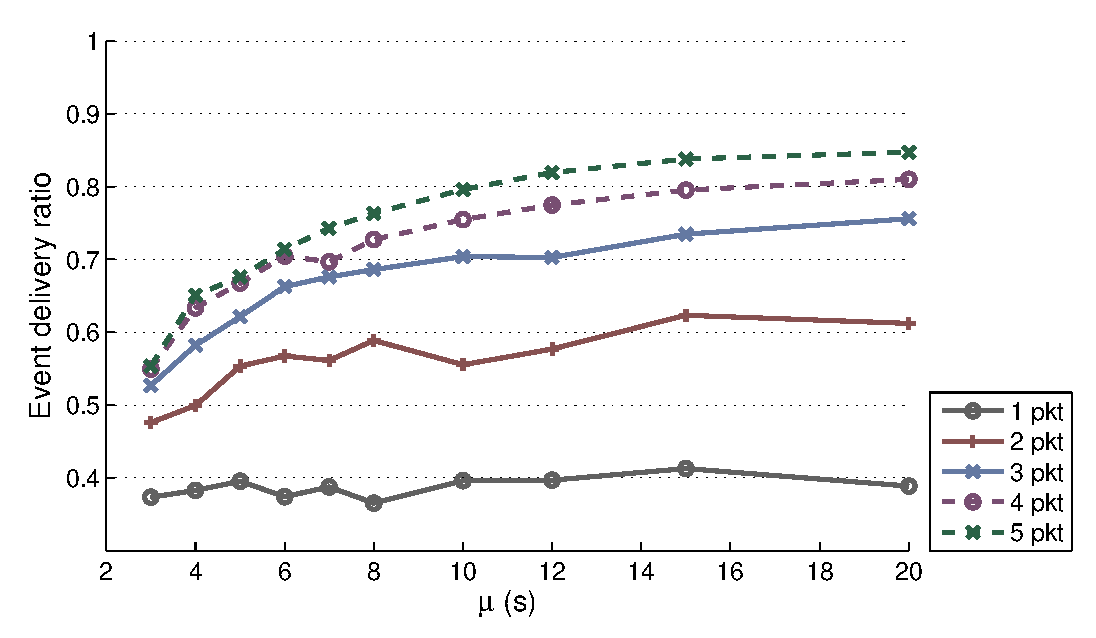
\includegraphics[width=\textwidth] {../../sw/pc/matlab/simulation-result/retrans-count-edr-250evt-pdr0.4.eps}
        \caption{}
    \end{subfigure} 
    \\
    \begin{subfigure}[t]{0.9\textwidth}
        \centering
        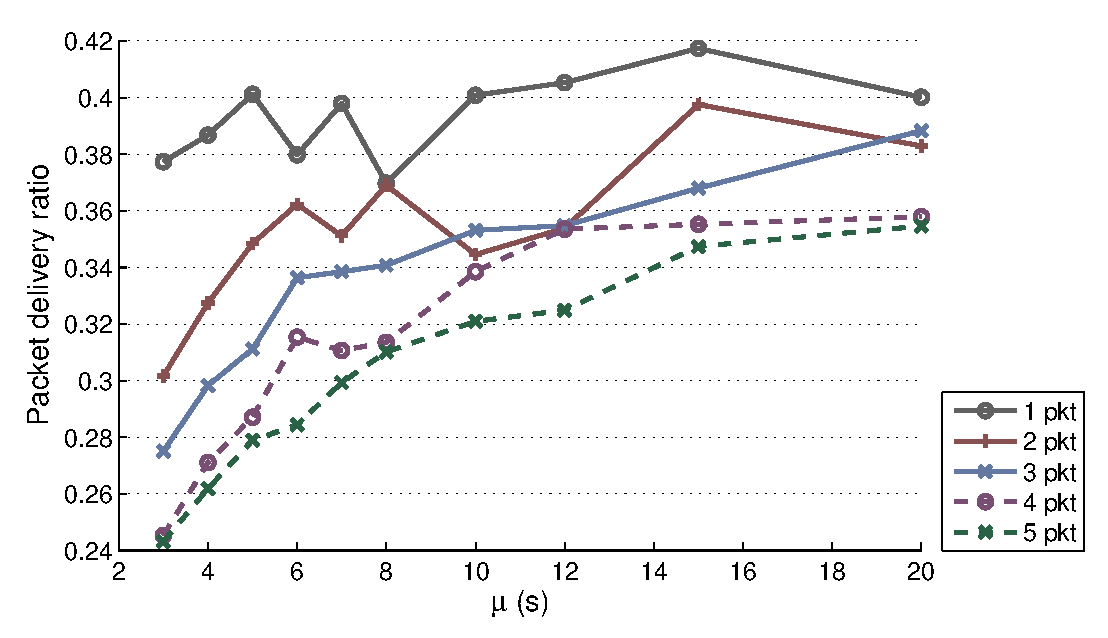
\includegraphics[width=\textwidth] {../../sw/pc/matlab/simulation-result/retrans-count-pdr-250evt-pdr0.4.eps}
        \caption{}
    \end{subfigure}
    \caption[$EDR$ and $PDR$ with different transmission redundancy, $PDR_0 = 0.4$]{Simulation results showing $EDR$(a) and $PDR$(b) with different number of retransmissions per event, at $PDR_0 = 0.4$}\label{fig:retrans-lambda-0.4}
\end{figure}


\begin{figure}[p]
    \centering
    \begin{subfigure}[t]{0.9\textwidth}
        \centering
        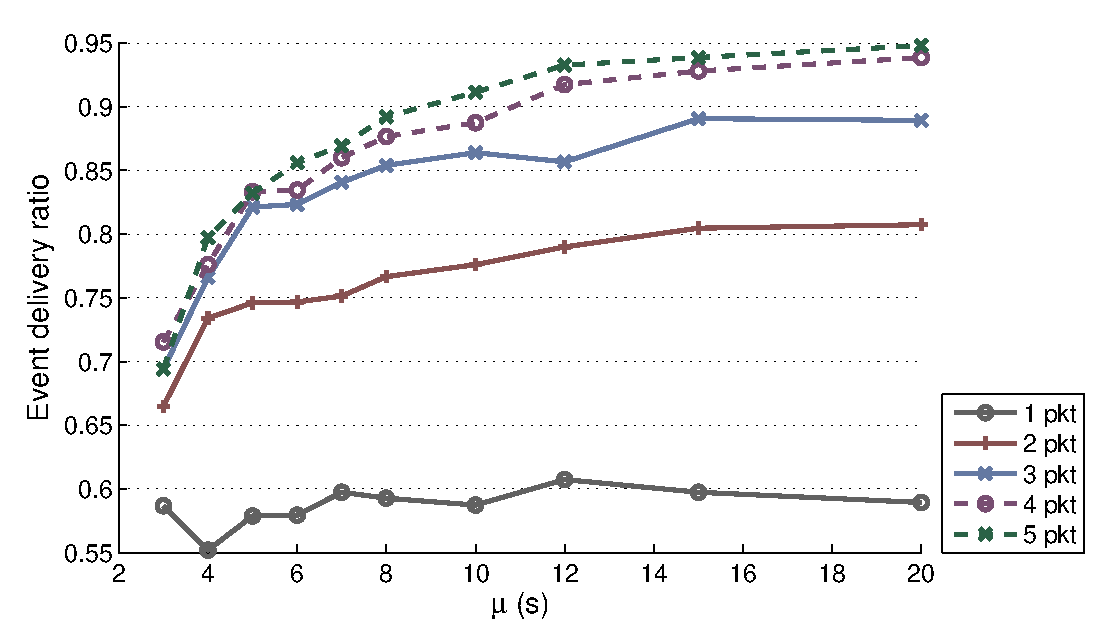
\includegraphics[width=\textwidth] {../../sw/pc/matlab/simulation-result/retrans-count-edr-250evt-pdr0.6.eps}
        \caption{}
    \end{subfigure} 
    \\
    \begin{subfigure}[t]{0.9\textwidth}
        \centering
        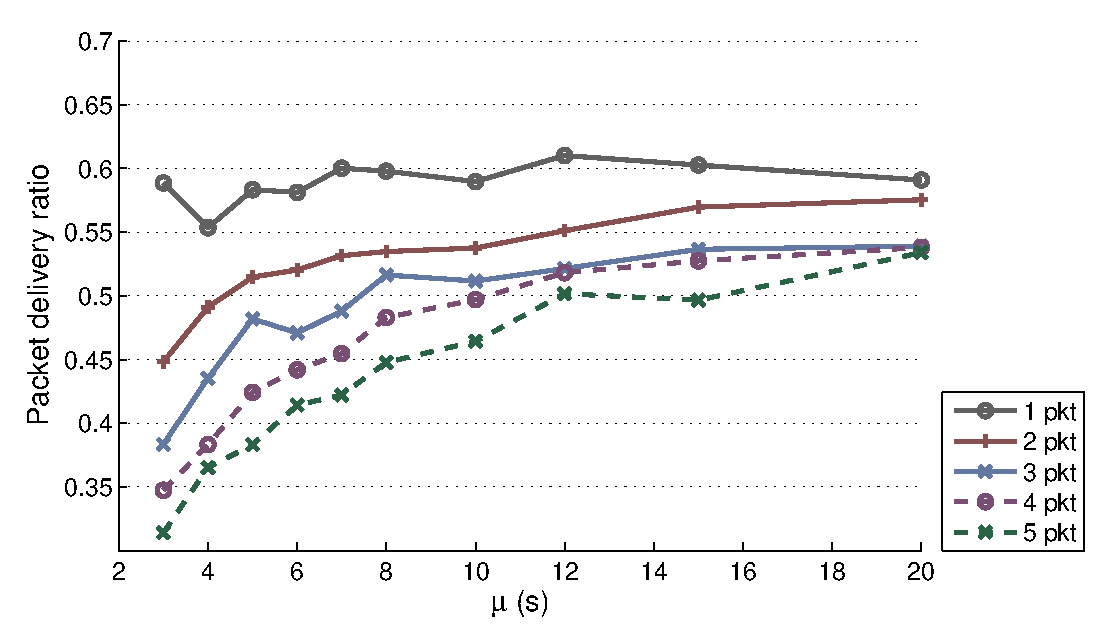
\includegraphics[width=\textwidth] {../../sw/pc/matlab/simulation-result/retrans-count-pdr-250evt-pdr0.6.eps}
        \caption{}
    \end{subfigure}
    \caption[$EDR$ and $PDR$ with different transmission redundancy, $PDR_0 = 0.6$]{Simulation results showing $EDR$(a) and $PDR$(b) with different number of retransmissions per event, at $PDR_0 = 0.6$}\label{fig:retrans-lambda-0.6}
\end{figure}


\begin{figure}[p]
    \centering
    \begin{subfigure}[t]{0.9\textwidth}
        \centering
        \includegraphics[width=\textwidth] {../../sw/pc/matlab/simulation-result/retrans-count-edr-250evt-pdr0.8.eps}
        \caption{}
    \end{subfigure} 
    \\
    \begin{subfigure}[t]{0.9\textwidth}
        \centering
        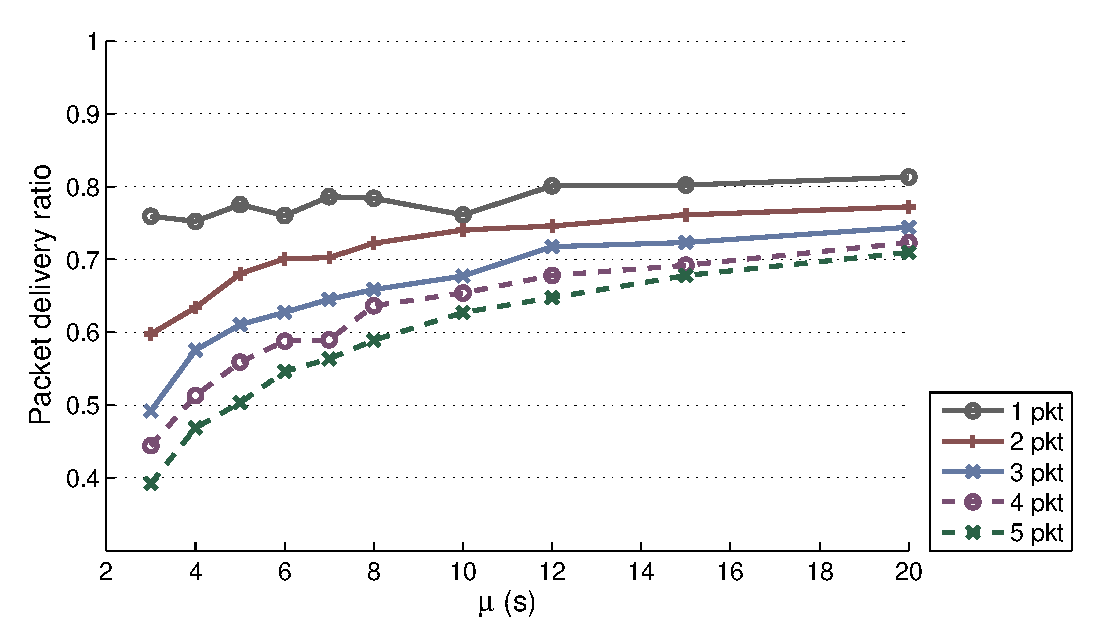
\includegraphics[width=\textwidth] {../../sw/pc/matlab/simulation-result/retrans-count-pdr-250evt-pdr0.8.eps}
        \caption{}
    \end{subfigure}
    \caption[$EDR$ and $PDR$ with different transmission redundancy, $PDR_0 = 0.8$]{Simulation results showing $EDR$(a) and $PDR$(b) with different number of retransmissions per event, at $PDR_0 = 0.8$}\label{fig:retrans-lambda-0.8}
\end{figure}


\begin{figure}[p]
    \centering
    \begin{subfigure}[t]{0.9\textwidth}
        \centering
        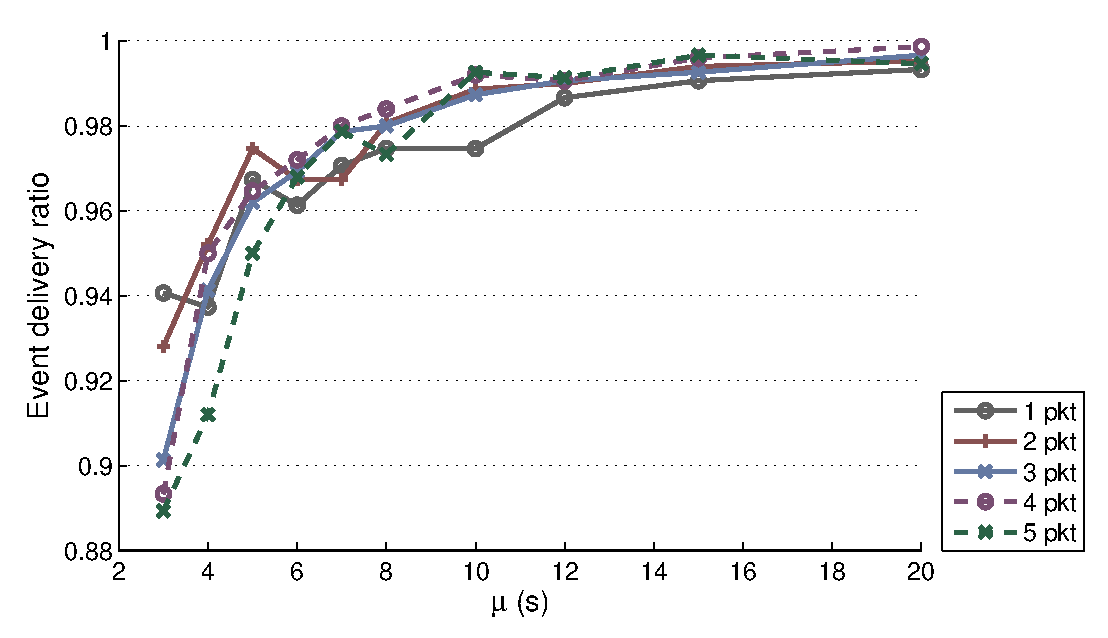
\includegraphics[width=\textwidth] {../../sw/pc/matlab/simulation-result/retrans-count-edr-250evt-pdr1.eps}
        \caption{}
    \end{subfigure} 
    \\
    \begin{subfigure}[t]{0.9\textwidth}
        \centering
        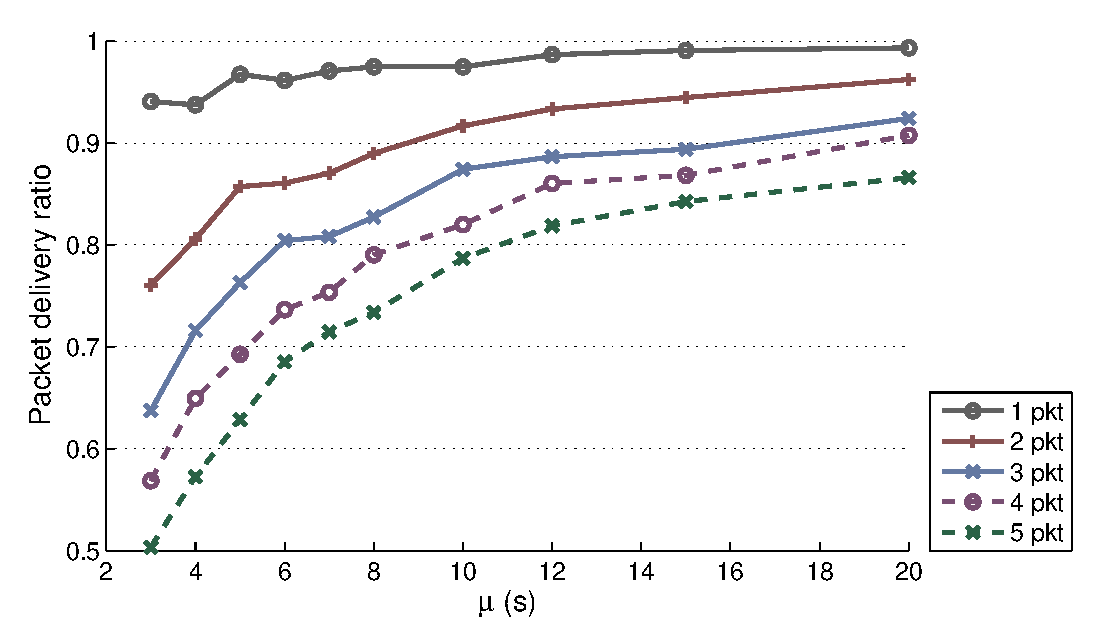
\includegraphics[width=\textwidth] {../../sw/pc/matlab/simulation-result/retrans-count-pdr-250evt-pdr1.eps}
        \caption{}
    \end{subfigure}
    \caption[$EDR$ and $PDR$ with different transmission redundancy, $PDR_0 = 1$]{Simulation results showing $EDR$(a) and $PDR$(b) with different number of retransmissions per event, at $PDR_0 = 1$}\label{fig:retrans-lambda-1}
\end{figure}

\begin{figure}[p]
    \centering
    \begin{subfigure}[t]{0.8\textwidth}
        \centering
        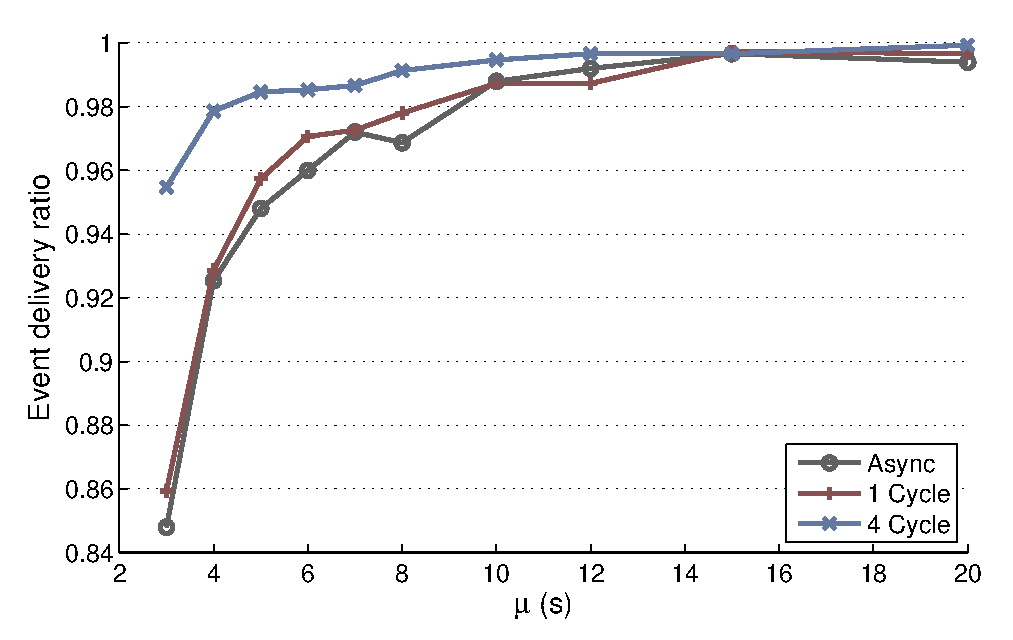
\includegraphics[width=\textwidth] {../../sw/pc/matlab/simulation-result/slotting-edr-250evt.eps}
        \caption{}
    \end{subfigure} 
    \\
    \begin{subfigure}[t]{0.8\textwidth}
        \centering
        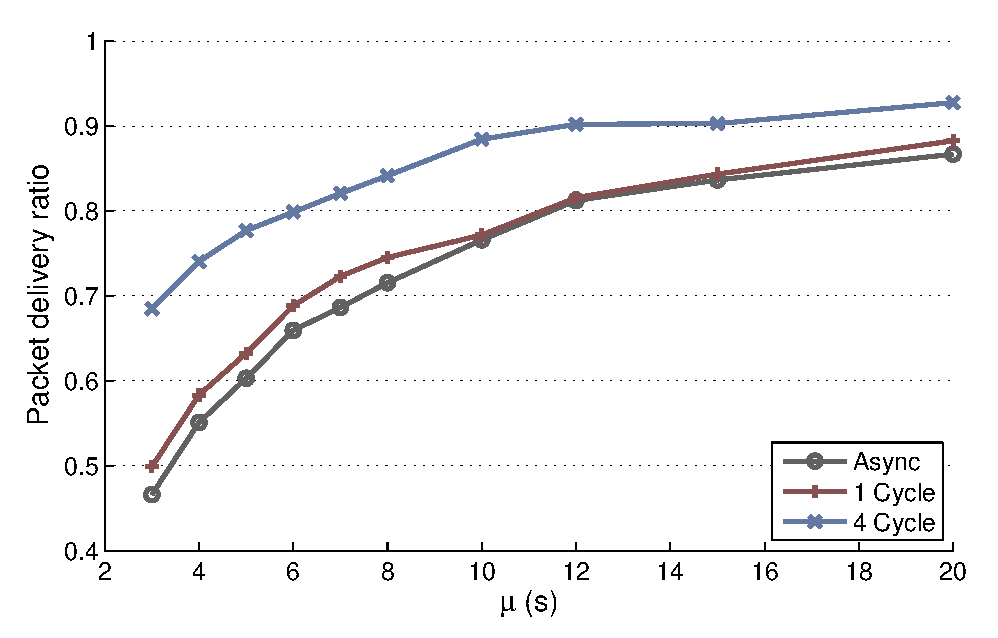
\includegraphics[width=\textwidth] {../../sw/pc/matlab/simulation-result/slotting-pdr-250evt.eps}
        \caption{}
    \end{subfigure}
    \caption[$EDR$ and $PDR$ with different timeslot alignment]{Simulation results showing $EDR$(a) and $PDR$(b) with different timeslot alignment}\label{fig:edr-pdr-slotting}
\end{figure}

When the events are dense, i.e. shorter $\mu$. Having multiple transmissions do not improve $EDR$, because the number of packets is multiplied, so does the chance of collision. When the events are sparse, the advantage of having multiple redundant transmissions becomes significant, especially with low $PDR_0$. This is more likely to be the case in real settings: sparse events, and some sensors have low $PDR_0$ because of long range or obstacles. 

We know that in computer networks, having packets fitted into timeslots which are fully aligned among senders can reduce collision and improve throughput, as in slotted ALOHA \cite{Roberts1975}. In our design, packets are synchronized to AC cycles. However, they are not fully aligned because each timeslot takes 4 AC cycles. Here, through simulation, we evaluate the difference in $EDR$ and $PDR$ with fully asynchronous, 1-cycle-synchronous and 4-cycle-synchronous (fully aligned) systems. 

The result in Fig.\ref{fig:edr-pdr-slotting} shows that synchronizing packets to AC cycles do have slight improvement on $EDR$ and $PDR$ compared to the case of fully asynchronous. On the other hand, having the packet slots fully aligned improves the delivery ratios significantly, compared to the other two cases. Currently, we can synchronize to one cycle by the zero-crossing circuit. We can not employ the fully-aligned scheme unless we add other hardware capabilities. Another way is to reduce packet length to less than one AC cycle, which means also raising transmitter power in order to get the same $PDR_0$. 

\subsection{Two-event collision test and Poisson distribution events}

We setup a small scale testbed so that we can test real hardwares with programmatically controllable events. We control the events through an extra microcontroller which is connected to a computer. The extra microcontroller, which is an mbed\footnote{http://mbed.org/}, is connected to each sensor with a wire. It toggles the wire to indicate events. The mbed is also connected to the computer with a USB emulated serial port. A perl script running on the computer can issue events to the sensors with the help of the mbed. 

The sensors run a slightly modified version of firmware, which enables them to receive events from the digital input pin, instead of using the AC current step detection. Nevertheless, the AC current step detection algorithms are still running, in order to emulate the timing of event detection as accurate as possible. The RF transmission code is unmodified. The sensors are plugged into AC sockets and powered by AC, so that the zero-crossing function is also working in the same way as it would in real deployment. 

We conduct a two-event collision test. Since all 5 transmissions of a single event can take up to 2.2s, any two events that happen within 2.2s on two different sensors are considered collided events. Note that two events that happen within 2.2 on a single sensor are not collided, because any pending retransmissions of the first event (flash event) are cancelled. 

\begin{figure}[htb]
  \centering
  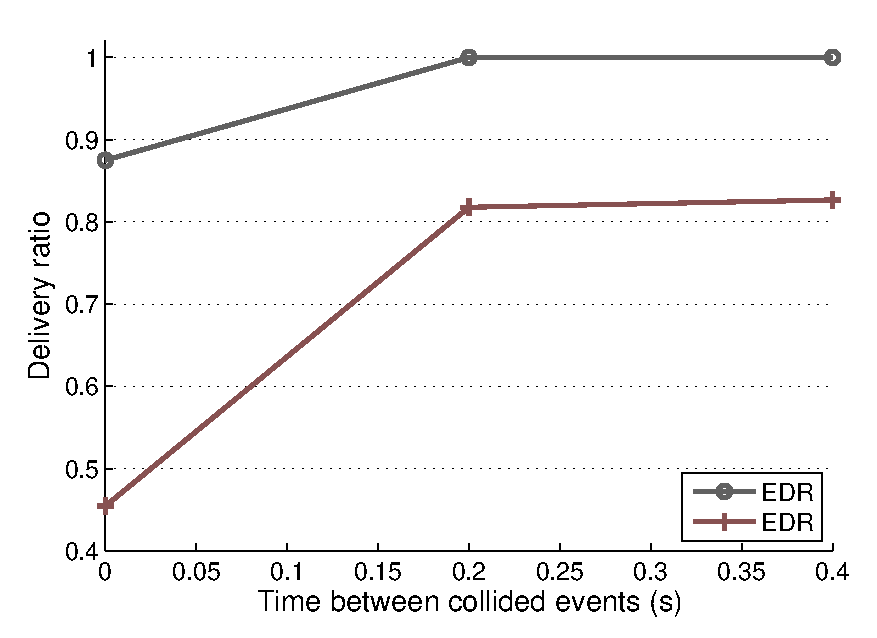
\includegraphics[width=0.7\textwidth]{../../sw/pc/matlab/testbed-result/collision}
  \caption{Two-event collision test result}
  \label{fig:collision}
\end{figure}

\begin{figure}[htb]
  \centering
  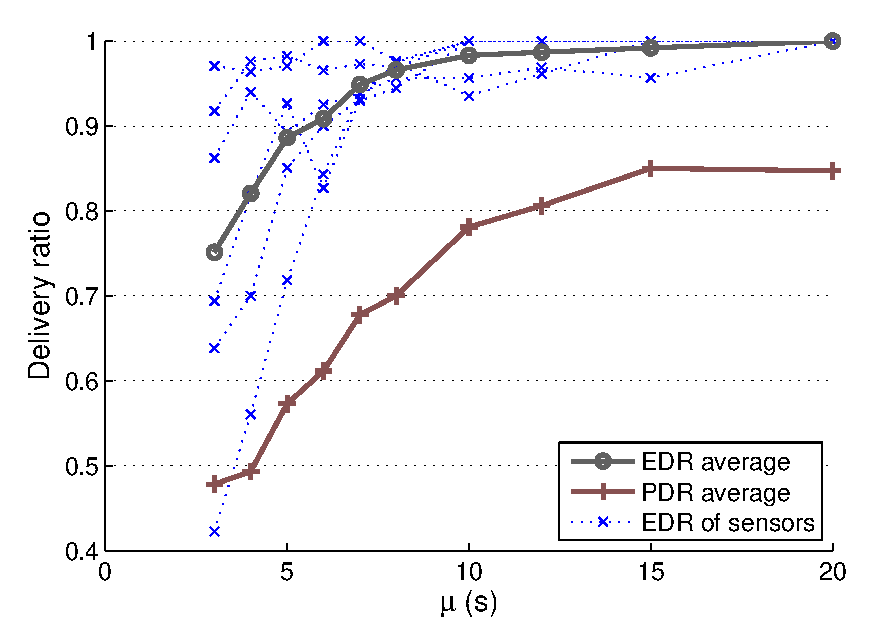
\includegraphics[width=0.7\textwidth]{../../sw/pc/matlab/testbed-result/poisson-5min}
  \caption{Poisson distribution events test}
  \label{fig:poisson-5min}
\end{figure}

In this test, we generate collided events two at a time for 100 times. In each testing set, the interval between each pair of collided events is fixed. Fig.\ref{fig:collision} shows the resulting $EDR$ and $PDR$. The plots show that $EDR$ becomes perfect when the interval between collided events are greater than 0.2s. In real cases, it is unlikely that two events happen at exactly the same time. Even if some appliances are highly correlated in term of their on-off states, such as a DVD player and a TV set, their turn-on time are not strictly aligned. Even in the extreme case of two strictly synchronous events, the system can still delivery them at a high probability of 88\%. 

Again, we use poisson distribution datasets on the testbed. The datasets are synthesized in the same way as described in the previous section, with $N = 6$, $\mu$ varying from 3 to 20. We limit the length of each dataset to 300 seconds long. Fig.\ref{fig:poisson-5min} shows the average $EDR$ and $PDR$, as well as the $EDR$ of each sensor separately. We can see that as the event density increases, some sensors are much worse than the others. This is because the transmission power differs among the sensors. The receiver has an automatic gain control (AGC) to tune the receiving signal strength. However, the AGC needs time to settle. When the transmission are too busy, the AGC can not accommodate all sensors fast enough. If the events are sparse, in the case of longer $\mu$, all sensor nodes have near perfect $EDR$. Again, even with $\mu=20$, the events are much more denser than a real setting. Appliances are very unlikely to be switched off and on within 20 seconds. 

\subsection{Evaluation in a real setting}

In this section, we provide the statistics of the sensor network with a dataset collected in a real setting. We have 21 sensors deployed in our lab, numbered \#1 through \#22. Details about the deployment are discussed in Chapter \ref{chap5}. \#10 is not deployed. \#16 is deployed, but there is no event during the time window of this dataset. \#20 is later removed. 

The dataset we used for the statistics contains data collected in 18 days. Note that in the real setting, lost packets and lost events are detected by purely analyzing the sequence number. This is accurate unless there are more than 16 successive packet loss, which is very rare. Fig.\ref{fig:real-edr-pdr} shows the $EDR$ and $PDR$ of each sensor. We can see that all sensors achieve almost perfect $EDR$, except for \#1. Detailed data are shown in Table \ref{tab:recvstat}.

\begin{figure}[htb]
  \centering
  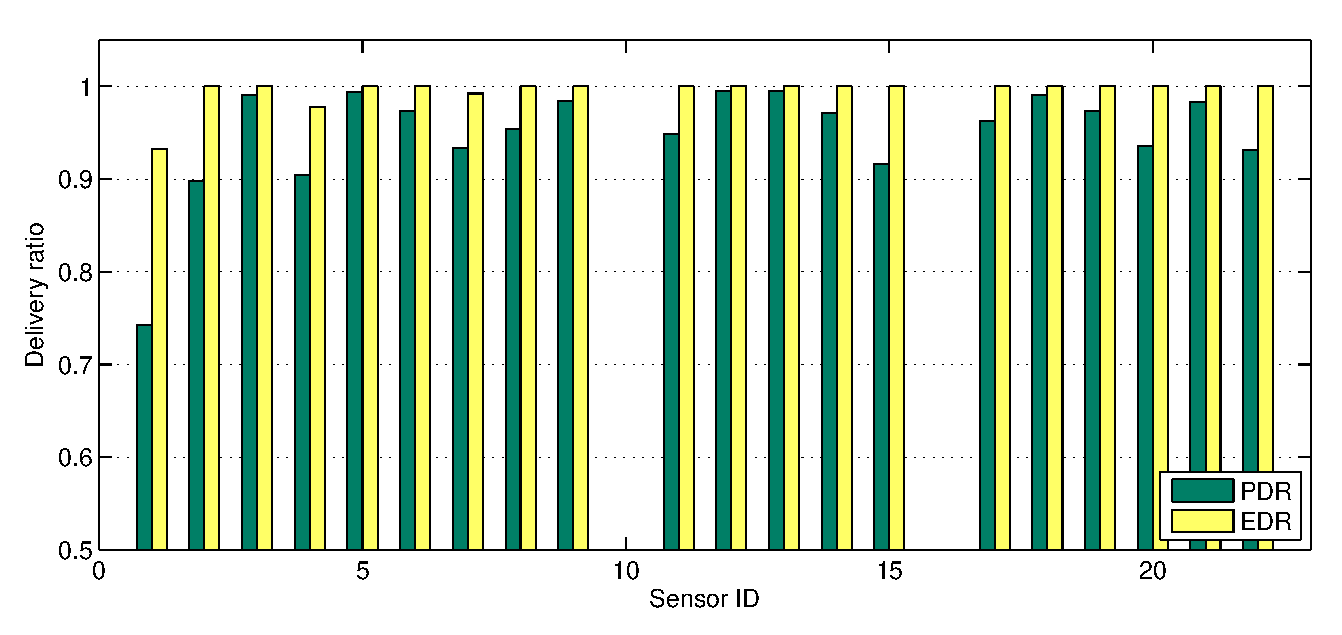
\includegraphics[width=\textwidth]{../../sw/pc/matlab/testbed-result/real}
  \caption{$EDR$ and $PDR$ in a real setting}
  \label{fig:real-edr-pdr}
\end{figure}

\begin{table}
  \centering
  \begin{tabular}{lcccc}
  \hline
  ID & RX Packets & TX packets & RX Events & TX Events \\
  \hline
1&      308     &    415    &      83     &     89\\
  2&       247    &     275   &       64    &      64\\
  3&       628    &     634   &      137    &     137\\
  4&       208    &     230   &       44    &      45\\
  5&       331    &     333   &       67    &      67\\
  6&        37    &      38   &        8    &       8\\
  7&     20364    &   21818   &     4534    &    4569\\
  8&       290    &     304   &       69    &      69\\
  9&       307    &     312   &       81    &      81\\
%  10&         0   &        0  &         0   &        0\\
  11&       354   &      373   &       81    &      81\\
  12&       216   &      217  &        54    &      54\\
  13&       438   &      440  &        88    &      88\\
  14&       134   &      138  &        30    &      30\\
  15&        55   &       60  &        12    &      12\\
  16&         0   &        0  &         0    &       0\\
  17&       255   &      265  &        54    &      54\\
  18&      1125   &    1135   &      227     &    227\\
  19&       146   &      150  &        30    &      30\\
  20&       452   &     483   &       97     &     97\\
  21&       586   &     596   &      120     &    120\\
  22&       270   &      290  &        58    &      58 \\ 
  \hline
  Total&    26751   &    28506   &     5938    &    5980 \\ 
  \hline
  \end{tabular}
  \caption{Sensor network delivery statistics in a real setting}
  \label{tab:recvstat}
\end{table}
